\section{Methodology}\label{methodology}

\subsection{Problem Formulation}
Our objective is to generate Sentinel-2 optical images from Sentinel-1 SAR observations. This task can be formulated as an image-to-image translation problem. Let $S \in \mathbb{R}^{H \times W \times 2}$ denote a Sentinel-1 image of spatial resolution $H \times W$ with two polarization channels (VV and VH), and let $O \in \mathbb{R}^{H \times W \times 12}$ denote the corresponding Sentinel-2 image with 12 spectral bands. Given $S$, the goal is to predict $O$ such that the generated image preserves the spatial structure from the SAR input while faithfully reconstructing the spectral information of the optical counterpart.

Formally, we aim to learn a mapping function
\[
f_\theta : \mathbb{R}^{H \times W \times 2} \rightarrow \mathbb{R}^{H \times W \times 12},
\]
parameterized by $\theta$, that minimizes the reconstruction error between the predicted optical image $\hat{O} = f_\theta(S)$ and the ground truth $O$. The optimization objective is expressed as
\[
\min_{\theta} \; L(f_\theta(S), O),
\]
where $L$ is the loss function. In this work, we adopt the Mean Absolute Error (MAE) loss:
\[
L(\hat{O}, O) = \frac{1}{H \cdot W \cdot 12} \sum_{i=1}^{H} \sum_{j=1}^{W} \sum_{c=1}^{12} \big| \hat{O}_{i,j,c} - O_{i,j,c} \big|.
\]

While Sentinel-1 captures structural and backscatter information that is robust to weather and lighting conditions, Sentinel-2 provides rich spectral information sensitive to surface reflectance properties. The main challenge of this task is the heterogeneity between SAR and optical data, as they capture different physical properties of the Earth's surface. The model must therefore learn a consistent mapping from radar backscatter to optical reflectance.  



\subsection{Proposed Architecture: Bidirectional Mamba Bridged UNet (BiMBU)}
We propose the Bidirectional Mamba Bridged UNet (BiMBU), an image-to-image translation architecture that integrates a convolutional U-Net structure with a Bidirectional Mamba (BiM) bottleneck for enhanced spatial feature extraction (cf.~\ref{fig:bimbu}). Given an input tensor $\mathbf{X} \in \mathbb{R}^{H \times W \times C_{in}}$, where spatial dimensions $H, W \in \{64, 128, 256\}$ and the number of input channels $C_{in} \in \{1, 2\}$, the model predicts an output tensor $\mathbf{\hat{Y}} \in \mathbb{R}^{H \times W \times C_{out}}$ with $C_{out} = 12$. The model is composed of three main parts: a convolutional encoder, a Mamba-based bottleneck, and a convolutional decoder.

\begin{figure*}
    \centering
    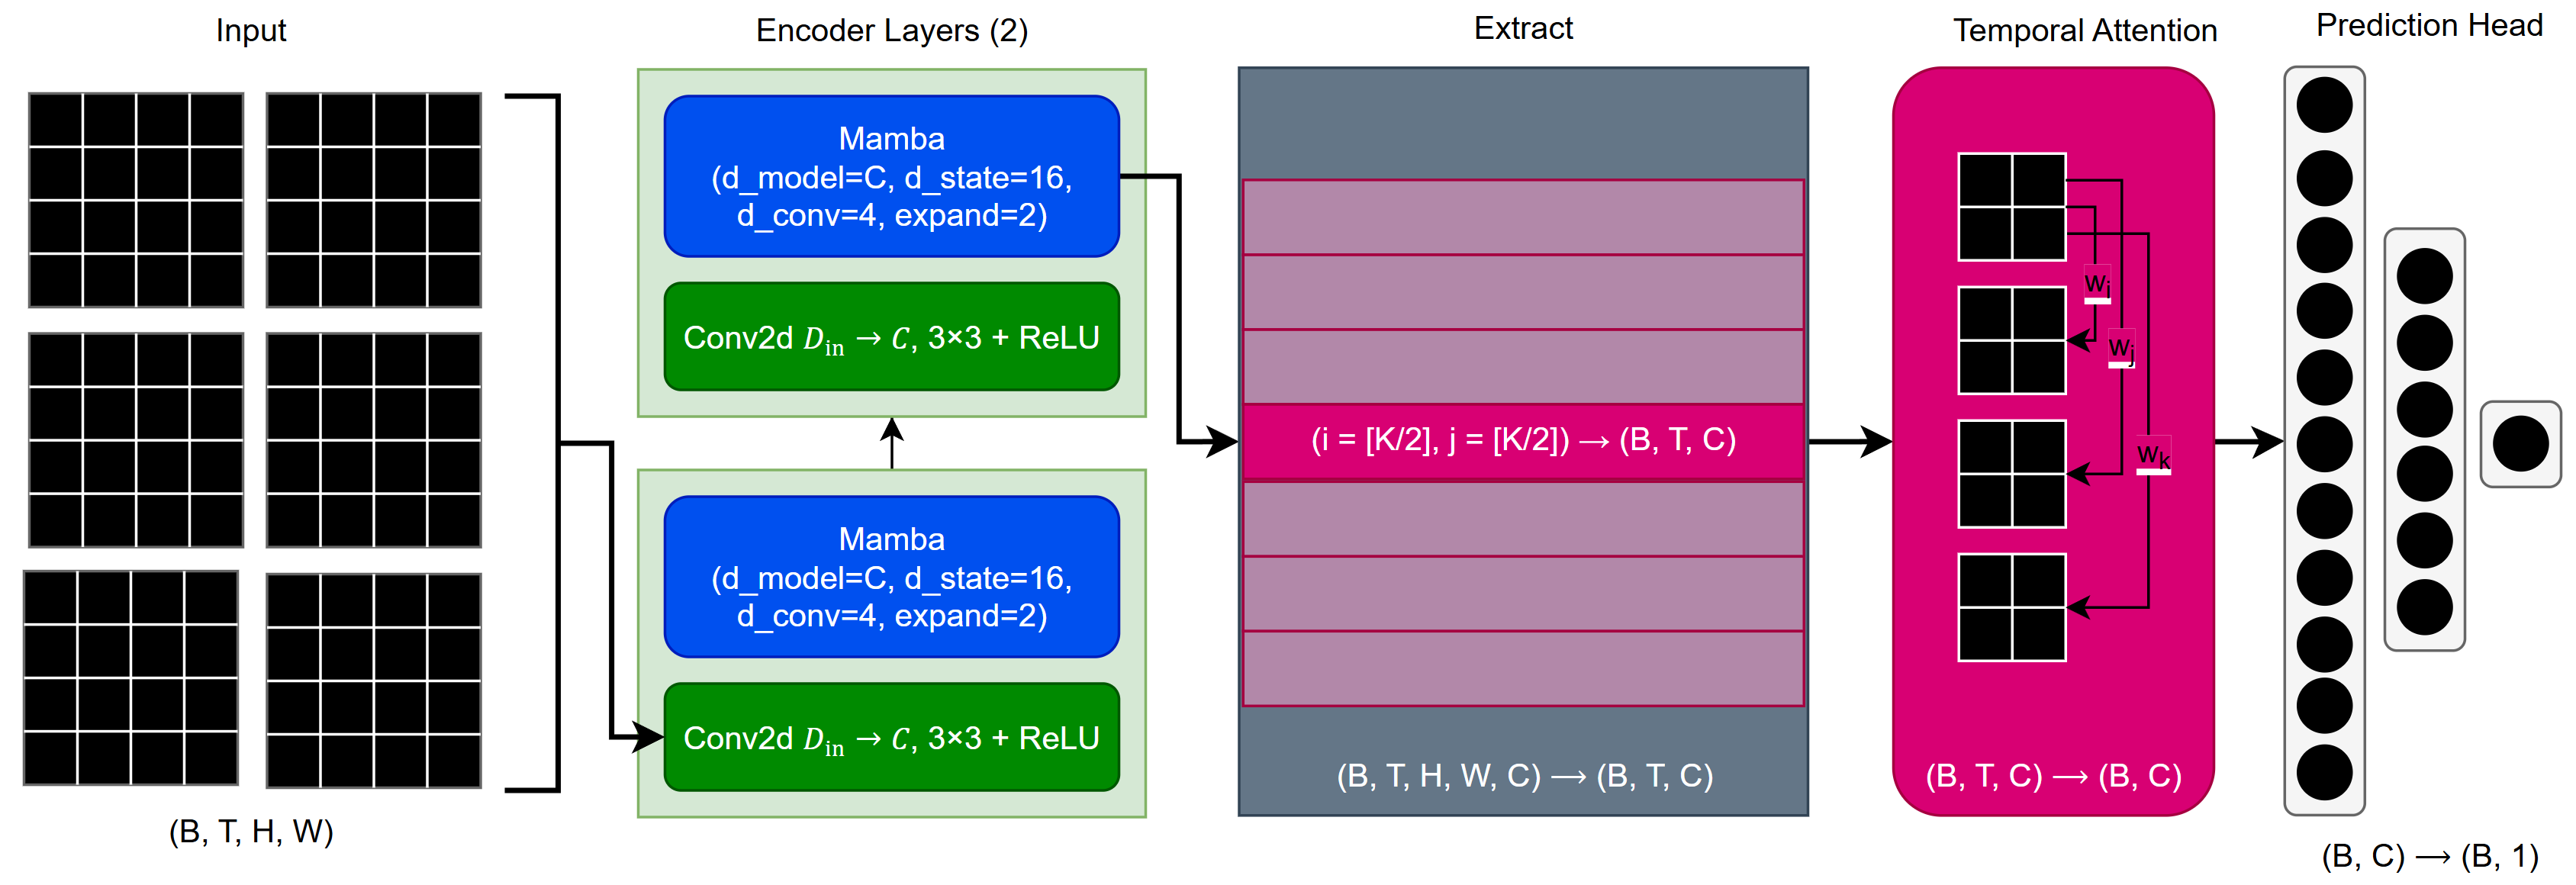
\includegraphics[width=\textwidth]{arch.png}
    \caption{Bidirectional Mamba Bridged UNet (BiMBU) Architecture}
    \label{fig:bimbu}
\end{figure*}

\subsubsection{Convolutional Encoder}
The encoder follows a standard U-Net downsampling path, consisting of four stages. Each stage comprises a convolutional block followed by a $2 \times 2$ max-pooling operation for downsampling. The convolutional block contains two 2D convolution layers, each followed by a Group Normalization and a GELU activation function. At each downsampling stage, the number of feature channels is doubled, allowing the model to learn increasingly abstract and high-level features while reducing spatial dimensions. High-resolution feature maps from each stage are preserved for later use in the decoder via skip connections.

\subsubsection{Bidirectional Mamba Bottleneck}
The bottleneck of the network serves to process the high-level features from the encoder. The input feature map $\mathbf{X}_{\text{enc}} \in \mathbb{R}^{B \times C \times H' \times W'}$ is flattened into a sequence of spatial tokens $\mathbf{X}_{\text{flat}} \in \mathbb{R}^{B \times (H'W') \times C}$. This sequence is then processed by the Bidirectional Mamba block, which contains two Mamba SSMs:
\begin{itemize}
    \item A \textbf{forward Mamba} processes the sequence as is.
    \item A \textbf{backward Mamba} processes a reversed version of the sequence.
\end{itemize}
The outputs from both Mamba models are concatenated and fused using a linear layer, allowing the model to capture long-range spatial dependencies from two directions. The Mamba SSM's ability to selectively retain and propagate information is particularly effective for modeling complex spatial relationships. The resulting fused features are then reshaped back to their original spatial dimensions, $\mathbb{R}^{B \times C \times H' \times W'}$.

\subsubsection{Convolutional Decoder}
The decoder reconstructs the high-resolution output image from the bottleneck features. It consists of three upsampling stages. In each stage, a $2 \times 2$ transposed convolution doubles the spatial dimensions of the feature map. The upsampled features are then concatenated with the corresponding high-resolution feature maps from the encoder path via skip connections. This concatenation is processed by a convolutional block identical to those in the encoder. This process allows the network to combine high-level, abstract features with fine-grained spatial details to produce a precise output.

\subsubsection{Output Head}
Finally, a $1 \times 1$ convolutional layer is applied to the output of the final decoder stage. This layer maps the feature channels to the desired number of output channels, $C_{out}=12$, producing the final output tensor $\mathbf{\hat{Y}} \in \mathbb{R}^{H \times W \times 12}$.



\subsection{Baseline Models}
We compare our proposed model BiMBU against the following baselines:

\begin{itemize}
  \item \textbf{Pix2Pix GAN}~\cite{isola2017image}: A conditional adversarial network for paired image-to-image translation, employing a U-Net generator and a PatchGAN discriminator. It combines reconstruction loss (L1) with adversarial loss to encourage both fidelity and realism in generated images.

  \item \textbf{Swin-UNet}~\cite{swinunet2023}: A purely Transformer-based U-shaped encoder–decoder architecture using hierarchical Swin Transformer blocks with shifted windows and skip-connections, enabling multi-scale context aggregation across spatial dimensions. 

  \item \textbf{U-Mamba}~\cite{umamba2024}: A hybrid encoder–decoder network integrating convolutional residual blocks with Mamba-based state-space modeling to capture both local features and long-range dependencies. Originally developed for biomedical image segmentation, U-Mamba’s architecture is adapted here for cross-modal remote-sensing translation.
\end{itemize}

